\documentclass[twocolumn,superscriptaddress,pre]{revtex4-1}

\usepackage[english]{babel}
\usepackage[utf8]{inputenc}
\usepackage{prettyref}
\usepackage{graphicx}
\usepackage{amsmath}
\usepackage{amssymb}

\usepackage[babel]{csquotes}
\usepackage[hidelinks]{hyperref} % load as last package

\DeclareMathOperator{\atan}{atan}


\begin{document}

\title{Casimir force between metallic mirrors}

\author{Michael Hartmann}
\affiliation{Universität Augsburg, Institut für Physik, 86135 Augsburg, Germany}

\date{\today}

\begin{abstract}
The Casimir free energy after Wick rotation depends on the dielectric function
on the imaginary axis. Here, we discuss how the dielectric function can be
rotated to the imaginary axis.
\end{abstract}

\maketitle

\section{Introduction}

The Casimir free energy in the plane-plane geometry is a function of the
separation $L$ between the two plates, the temperature $T$ and the optical
properties of the plates
\begin{equation}
{\cal F} = {\cal F}\left(L,T,\epsilon(i\omega)\right) \,.
\end{equation}
Due to the Wick rotation, the dielectric function is evaluated for imaginary
frequencies. The dielectric function on the imaginary axis is connected with
the imaginary part of the dielectric function by the Kramers-Kronig relations.

Here, we show how to compute the dielectric function on the imaginary axis from
optical data, and discuss problems related to the extrapolation of the
experimental data for small frequencies. The general idea was discussed in
\cite{Lambrecht2000}, a more detailed analysis about the dependence of the
optical properties on the preparation and the variation of the Casimir force
calculated with the use of different optical data can be found in
\cite{Pirozhenko2006}.

\section{Kramers-Kronig relations}

\begin{figure}
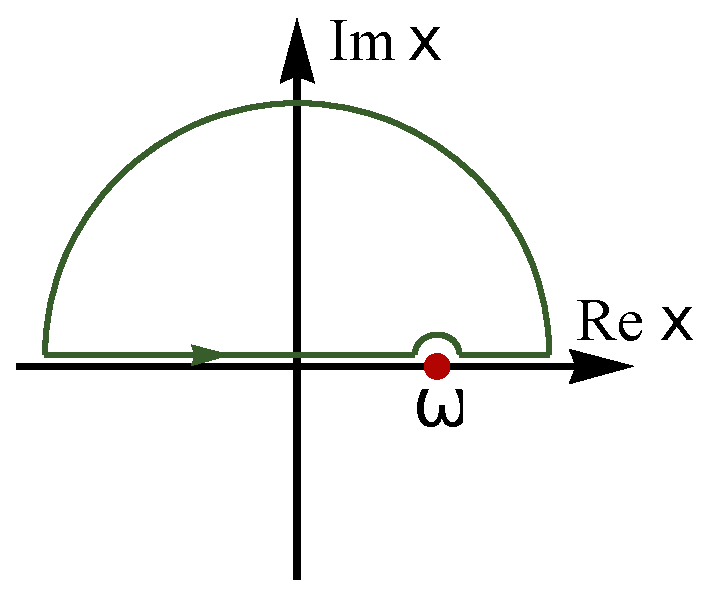
\includegraphics[width=0.5\columnwidth]{img/contour.eps}
\caption{Contour $\cal C$ used to derive the Kramers-Kronig relations.}
\label{fig:contour}
\end{figure}

The Kramers-Kronig relations connect the real and imaginary parts of a complex
function that is analytic in the upper half-plane. Let $\chi=\chi'+i\chi''$ be
analytic in the closed upper half-space, $\chi'$ and $\chi''$ are real, and
$\chi(x)$ vanishes faster than $|x|^{-1}$ as $x\to\infty$. Then the line
integral with the contour $\cal C$ sketched in Fig. \ref{fig:contour} vanishes,
\begin{equation}
\oint_{\cal C} \mathrm{d}x \frac{\chi(x)}{x-\omega} = \lim_{\epsilon\to0^+} \int_{-\infty}^\infty \mathrm{d}x \frac{\chi(x)}{x-\omega+i\epsilon} = 0 \,.
\end{equation}
Substituting $z=x-\omega$ and separating real and imaginary parts, we find
\begin{equation}
0 = \lim_{\epsilon\to0^+}\int_{-\infty}^\infty \mathrm{d}z \frac{z \chi(z+\omega)}{z^2+\epsilon^2} - i\pi \lim_{\epsilon\to0^+} \int_{-\infty}^\infty \mathrm{d}z \frac{\epsilon \chi(z+\omega)}{\pi(z^2+\omega^2)} \,.
\end{equation}
The first term on the right-hand side corresponds to a principal value, while
the second term in the limit $\epsilon\to0^+$ becomes a Dirac delta function,
\begin{equation}
0 = {\cal P} \int_{-\infty}^\infty \mathrm{d}z \frac{\chi(z+\omega)}{z} - i\pi \chi(\omega) \,.
\end{equation}
After resubstituting and splitting up real and imaginary parts, we find the
famous Kramers-Kronig relations:
\begin{align}
\label{eq:KK1}
\chi'(\omega)  &= +\frac{1}{\pi} {\cal P} \int_{-\infty}^\infty \mathrm{d}x \frac{\chi''(x)}{x-\omega} \\
\label{eq:KK2}
\chi''(\omega) &= -\frac{1}{\pi} {\cal P} \int_{-\infty}^\infty \mathrm{d}x \frac{\chi'(x) }{x-\omega}
\end{align}


\section{Rotating $\epsilon(\omega)$ to the imaginary axis}

Here, we focus on the dielectric function
\begin{equation}
\epsilon(\omega)=\chi(\omega)+1 \,.
\end{equation}
In the time-domain, the dielectric function $\epsilon(t)$ is real, which implies the symmetry $\epsilon(-\omega) = \epsilon^*(\omega)$ in the
frequency-domain. For this reason,
$\epsilon'(\omega)$ is an even function while $\epsilon''(\omega)$ is an odd
function. Using the Kramers-Kronig relation \eqref{eq:KK2}, we find that the
imaginary part of $\epsilon(i\omega)$ vanishes, because the integrand is odd
with respect to $x$,
\begin{equation}
\epsilon''(i\omega) = - \frac{1}{\pi} \int_{-\infty}^\infty \mathrm{d}x \frac{\epsilon'(x)-1}{x-i\omega} = 0 \,.
\end{equation}
The real part is readily evaluated using \eqref{eq:KK1}
\begin{equation}
\epsilon'(i\omega)-1 = \frac{1}{\pi} \int_{-\infty}^\infty \mathrm{d}x \frac{x\epsilon''(x)}{x^2+\omega^2} + \frac{i\omega}{\pi} \int_{-\infty}^\infty \mathrm{d}x \frac{\epsilon''(x)}{x^2+\omega^2} \,. 
\end{equation}
The integrand of the first integral on the right-hand side is even, and the
second integral vanishes, because its integrand is odd. Thus, we find
\begin{equation}
\epsilon(i\omega)-1 = \frac{2}{\pi} \int_0^\infty \mathrm{d}x \frac{x\epsilon''(x)}{x^2+\omega^2}
\end{equation}
for the dielectric function on the imaginary axis.

So, the dielectric function on the imaginary axis $\epsilon(i\omega)$ can be
computed from the imaginary part of $\epsilon''(\omega)$. However,
$\epsilon''(\omega)$ is only available in a finite interval
$\omega_\mathrm{min} \le \omega \le \omega_\mathrm{max}$. Typical values are $\omega_\mathrm{min} \sim 0.05\,$eV
and $\omega_\mathrm{max} \sim 10^4\,$eV, where $1\,\mathrm{eV}=1.519\,$rad/s.
We split up the
integral in three contributions and discuss each integral separately:
\begin{align}
\nonumber
\epsilon(i\omega)-1 =&
\frac{2}{\pi} \int_0^{\omega_\mathrm{min}} \mathrm{d}x \frac{x\epsilon''(x)}{x^2+\omega^2} +
\frac{2}{\pi} \int_{\omega_\mathrm{min}}^{\omega_\mathrm{max}} \mathrm{d}x \frac{x\epsilon''(x)}{x^2+\omega^2} \\
&+\frac{2}{\pi} \int_{\omega_\mathrm{max}}^\infty \mathrm{d}x \frac{x\epsilon''(x)}{x^2+\omega^2} \equiv \epsilon_1 + \epsilon_2 + \epsilon_3
\end{align}

\begin{itemize}
\item As $\epsilon''(\omega_\mathrm{max}) \sim 5\times10^{-6}$, the contribution
from $\epsilon_3$ is negligible.
\item The integral $\epsilon_2$ can be evaluated using numerical quadrature.
Typically, in this domain many points are available and the integration causes
no problems. Here, we use Simpson quadrature to evaluate the integral.
\item No data is available for small frequencies and the computation of
$\epsilon_1$ relies on an extrapolation of the optical data. Metals like
gold are well described by the Drude model
\begin{equation}
\label{eq:drude}
\epsilon^D(\omega) = 1 - \frac{\omega_P^2}{\omega(\omega+i\gamma)},
\end{equation}
where $\omega_P \sim 9\,$eV is the Plasma frequency and $\gamma \sim 35\,$meV
is related to dissipation. Using the Drude model, the integral becomes
\begin{equation}
\epsilon_3 = \frac{2}{\pi} \frac{\omega_P^2}{\omega^2-\gamma^2} \left[ \atan\left(\frac{\omega_\mathrm{min}}{\gamma}\right) - \frac{\gamma}{\omega} \atan\left(\frac{\omega_\mathrm{min}}{\omega}\right)\right] \,.
\end{equation}
The value of $\epsilon_1$ depends sensitively on the plasma frequency
$\omega_P$.
\end{itemize}

\section{Optical data}

\begin{table}
\begin{center}
\begin{tabular}{|ll|l|l|}
\hline
source & preparation & $\omega_P$ (eV) & $\gamma$ (meV) \\
\hline
\hline
Palik \cite{Palik1995,Pirozhenko2006} & & $7.50\pm0.02$ & $61\pm0.7$ \\
\hline
Svetovoy \cite{Svetovoy2008} & $400\,$nm/Si & $6.82\pm0.08$ & $40.5\pm2.1$ \\
                             & $200\,$nm/Si & $6.83\pm0.15$ & $39.5\pm4.4$ \\
                             & $100\,$nm/Si & $7.84\pm0.07$ & $49.0\pm2.1$ \\
                             & $120\,$nm/Si & $8.00\pm0.16$ & $35.7\pm5.1$ \\
                             & $120\,$nm/mica & $8.38\pm0.08$ & $37.1\pm1.9$ \\
\hline
Olmon \cite{Olmon2012} & EV & $8.5\pm0.5$ & $47$ \\
                       & TS & $8.8\pm0.05$ & $50$ \\
                       & SC & $8.1\pm0.8$ & $47$ \\
\hline
\end{tabular}
\end{center}
\caption{Plasma frequency $\omega_P$ and dissipation $\gamma$ for
different samples of gold in different experiments. The data is given by
\cite{Palik1995,Olmon2012,Svetovoy2008}.  The values for $\omega_P$ and
$\gamma$ for Palik's Handbook data were obtained in \cite{Pirozhenko2006},
while in \cite{Lambrecht2000} $\omega_P=9\,$eV and $\gamma=35\,$meV was found.}
\label{tab:gold}
\end{table}

\begin{figure}
\includegraphics[width=0.95\columnwidth]{img/eps.pdf}
\caption{Imaginary part of the dielectric function $\epsilon(\omega)$ for the
data of Palik \cite{Palik1995}, and the experiments by Olmon \cite{Olmon2012}
and Br\"andli \cite{Brandli1972}.}
\label{fig:eps}
\end{figure}

\begin{figure}
\includegraphics[width=0.95\columnwidth]{img/eps_imag.pdf}
\caption{Dielectric function for imaginary frequencies, $\epsilon(i\omega)$
obtained using Palik's optical data, and a compination of Olmon (SC) for small
and Palik's data for high frequencies.}
\label{fig:eps_imag}
\end{figure}

\begin{figure}
\includegraphics[width=0.7\columnwidth]{img/ratio.pdf}
\caption{Ratio of the integral $\epsilon_1$ and the total contribution $\epsilon_1+\epsilon_2$. The contribution of $\epsilon_3$ is negligibly small.}
\label{fig:ratio}
\end{figure}

\begin{figure}
\includegraphics[width=0.7\columnwidth]{img/diff.pdf}
\caption{Ratio of the force (PFA) for $R=100\,\mu$m and $T=300\,$K using the optical data from Palik \cite{Palik1995} and Olmon \cite{Olmon2012}.}
\label{fig:diff}
\end{figure}

There are many different experiments that measured the dielectric function of
gold. Often, the handbook data edited by \textsc{Palik} is used.
\cite{Palik1995}. \textsc{Olmon} et al.\ measured the dielectric function
$\epsilon(\omega)$ for evaporated (EV, 200\,nm thick film deposited by
evaporation onto a soda-lime glass substrate), template-stripped (TS, 200\,nm
film deposited onto a clean silicon substrate in the same evaporation run), and
single-crystal (SC, Au(111), thickness 1\,mm, diameter 10\,mm) gold in the range
from 0.04 to 4.14\,eV \cite{Olmon2012}. \textsc{Svetovoy} et al.\ measured five
gold films prepared by Au deposition on cleaned (100) Si or mica substrate with
varying thickness \cite{Svetovoy2008}.

The imaginary part of the dielectric function $\epsilon''(\omega)$ by Palik
\cite{Palik1995}, and the experiments by Olmon et al.\ \cite{Olmon2012} and
Br\"andli et al.\ \cite{Brandli1972} are shown in Fig.  \ref{fig:eps}. The
resulting dielectric function for imaginary frequencies $\epsilon(i\omega)$ is
plotted in Fig. \ref{fig:eps_imag}. The computed dielectric functions for
imaginary frequencies differ depending on the optical data used. The
simple Drude model \eqref{eq:drude} is in good agreement with the dielectric
function obtained by the optical data up to frequencies of $\sim 1\,$eV when
interband transitions become important.

Notably, the experiments find rather different values for the plasma frequency
$\omega_P$ and the dissipation rate $\gamma$, see Table \ref{tab:gold}. As the
value of $\epsilon_1$ depends sensitively on the value of the plasma frequency, high
accuracy in Casimir experiments requires a precise knowledge of the plasma
frequency. In particular, low Matsubara frequencies depend strongly on the
extrapolation, because for frequencies $\omega \lesssim 3\,$eV the contribution
of $\epsilon_1$ is dominant, as can be seen in Fig. \ref{fig:ratio}. In
contrast, the dependence of the dielectric function and the Casimir force on
$\gamma$ is typically weak.

The Casimir force may vary up to about $5\%$ at shortest distances depending
on the optical data used \cite{Pirozhenko2006}.
In Fig. \ref{fig:diff} we plot the ratio
of thethe  Casimir force for radius $R=100\,\mu$m at room-temperature $T=300\,$K
using the dielectric function obtained by Palik, and a combination of Olmon for
small and Palik for high frequencies. The difference of both dielectric
functions is quite big, because the plasma frequency for Palik is
$\omega_P=9\,$eV, and for Olmon it is $\omega_P=8.45\,$eV.


\section{Window functions}

In order to decrease the contribution of $\epsilon_1$,
\textsc{Bimonte} proposed to \cite{Bimonte2010}
to alter the Kramers-Kronig relations by a window function $f(x)$ \cite{Bimonte2010}. More precisely,
using the same derivation as before for $\chi(x)=f(x)[\epsilon(x)-1]$ one finds
\begin{equation}
\epsilon(i\omega)-1 = \frac{2}{\pi f(i\omega)} \int_0^\infty \mathrm{d}x \frac{x}{x^2+\omega^2} \mathrm{Im}\left\{ f(x)\left[\epsilon(x)-1\right] \right\} \,.
\end{equation}
The window function $f(x)$ can now be chosen in such a way that it suppresses
the contributions of $\epsilon_1$. However, it was pointed out in \cite{Shpak2011}
that the use of a window function can in some cases distort the Casimir force
calculations.

\section{Conclusion}

The dielectric function at imaginary frequencies $\epsilon(i\omega)$ depends on
the optical data used. The optical data, on the other hand, strongly depends on
the preparation. The plasma frequency may range from about about 8 to $9\,$eV
which gives a very different contribution from $\epsilon_1$. The difference may yield
to a deviation of several percent in the Casimir force.

``When we are speaking about a precise comparison between theory and experiment for the Casimir
force at the level of 1\% or better, there is no such material as gold in general any more.
There is only a gold sample prepared under definite conditions." \cite{Pirozhenko2006}

\begin{thebibliography}{99}

\bibitem{Lambrecht2000}
A. Lambrecht and S. Reynaud,
Casimir force between metallic mirrors,
Eur. Phys. J. D. \textbf{8}, 309-318 (2000).

\bibitem{Palik1995}
In \textit{Handbook of Optical Constants of Solids},
edited by E. D. Palik (Academic Press, New York, 1995)

\bibitem{Olmon2012}
R. L. Olmon, B. Slovick, T. W. Johnson, D. Shelton, S-H Oh, G. D. Boreman, and M. B. Raschke,
Optical dielectric function of gold,
Phys. Rev. B \textbf{86}, 235147 (2012)

\bibitem{Svetovoy2008}
V. B. Svetovoy, P. J. van Zwol, G. Palasantzas, and J. Th. M. De Hosson,
Optical properties of gold films and the Casimir force,
Phys. Rev. B. \textbf{77}, 035439 (2008)

\bibitem{Brandli1972}
G. Brandli and A. J. Sievers,
Phys. Rev. B 5, 3550 (1972)

\bibitem{Bimonte2010}
G. Bimonte,
Generalized Kramers-Kronig transform for Casimir effect computations,
Phys. Rev. A. \textbf{81}, 062501 (2010)

\bibitem{Shpak2011}
O. Shpak and G. Pasantzas,
Analysis of Casimir force with window functions: Kramers-Kronig general approach for real measured dielectric data,
Phys. Rev. A. \textbf{84}, 044501 (2011)

\bibitem{Pirozhenko2006}
I. Pirozhenko, A. Lambrecht, and V. B. Svetovoy,
Sample dependence of the Casimir force,
New J. Phys. \textbf{8}, 238 (2006)

\end{thebibliography}

\end{document}
